\begin{pastexam}[label={px:ncku-113-cce-18}]{成大電通所 113 學年度 簡答題第 9 題}
（簡答）

(5 pts) We can search a number by rank in a binary search tree if we add an additional
information to each node. Please show the number of comparisons before we can find the 4-th
smallest values in the right tree and give the information of each node to complete the
procedure.

\begin{center}
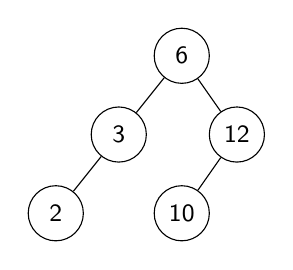
\begin{tikzpicture}[v/.style={draw,circle,minimum size=0.7cm,inner sep=0pt,font=\sffamily\small}]
  \node[v] (6) at (0,0) {6};
  \node[v] (3) at (-0.8,-1) {3};
  \node[v] (12) at (0.7,-1) {12};
  \node[v] (2) at (-1.6,-2) {2};
  \node[v] (10) at (0,-2) {10};
  \draw (6)--(3) (6)--(12) (3)--(2) (12)--(10);
\end{tikzpicture}
\end{center}
\end{pastexam}

\begin{pastsoln}
``the right tree'' 指原卷印在題目右邊的那棵樹（上圖）。 第 $4$ 小是 $10$，要走過 $6$、$12$、$10$
三個節點，各和 $k$ 比較一次，共 $3$ 次比較。

\textbf{每個節點加的資訊}：子樹大小 $\mathit{size}$，也就是以它為根的子樹有幾個節點
（資結書第~9.4~節）：
\begin{center}
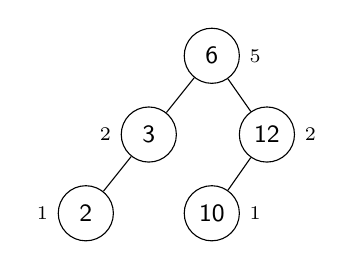
\begin{tikzpicture}[v/.style={draw,circle,minimum size=0.7cm,inner sep=0pt,font=\sffamily\small},
  sz/.style={font=\scriptsize}]
  \node[v,label={[sz]0:5}] (6) at (0,0) {6};
  \node[v,label={[sz]180:2}] (3) at (-0.8,-1) {3};
  \node[v,label={[sz]0:2}] (12) at (0.7,-1) {12};
  \node[v,label={[sz]180:1}] (2) at (-1.6,-2) {2};
  \node[v,label={[sz]0:1}] (10) at (0,-2) {10};
  \draw (6)--(3) (6)--(12) (3)--(2) (12)--(10);
\end{tikzpicture}
\end{center}
（節點旁的小字是 $\mathit{size}$：$x.\mathit{size} = x.\mathit{left}.\mathit{size} +
x.\mathit{right}.\mathit{size} + 1$，空子樹算 $0$。）

\textbf{找第 $k$ 小}（資結書虛擬碼~9.8 的 \proc{Tree-Select}）：在節點 $x$，
$r = x.\mathit{left}.\mathit{size} + 1$ 是 $x$ 在目前這棵子樹裡的名次。 $k = r$ 就是 $x$；
$k < r$ 往左找第 $k$ 小；$k > r$ 往右找第 $k - r$ 小。 找第 $4$ 小：
\begin{center}
\begin{tabular}{ccccl}
\toprule
步 & $x$ & $k$ & $r$ & 動作 \\
\midrule
1 & 6 & 4 & $2 + 1 = 3$ & $k > r$，$k \gets 4 - 3 = 1$，往右 \\
2 & 12 & 1 & $1 + 1 = 2$ & $k < r$，往左 \\
3 & 10 & 1 & $0 + 1 = 1$ & $k = r$，回傳 $10$ \\
\bottomrule
\end{tabular}
\end{center}
由小到大是 $2, 3, 6, 10, 12$，第 $4$ 小確實是 $10$。

比較次數的算法：每個走過的節點拿 $k$ 和 $r$ 做一次三向比較（$=$、$<$、$>$），共 $3$ 次。 如果
把虛擬碼裡的「$k = r$?」「$k < r$?」分開算，則是 $2 + 2 + 1 = 5$ 次。 作答時寫清楚採用哪一種
算法。 不管哪一種，只走一條從根往下的路徑，時間是 $O(h)$，$h$ 是樹高。
\end{pastsoln}
